\documentclass[10pt,twocolumn]{article}

% ---- packages ----
\usepackage[margin=0.75in]{geometry}
\usepackage{graphicx}
\usepackage{booktabs}
\usepackage{amsmath}
\usepackage{xcolor}
\usepackage{caption}
\usepackage{subcaption}
\usepackage[hidelinks]{hyperref}
\usepackage{float}
\graphicspath{{figures/}}
\captionsetup{font=small}
\setlength{\parskip}{2pt}

% ---- title ----
\title{\vspace{-1.5em}\textbf{Surface Style is Coachable, the Stylometric Signature is Not:\\
Detecting LLM Imitation of Student Discussion Writing}}
\author{Team \emph{[nickname]} --- COSE471 Data Science, Korea University\\
\small Member A, Member B, Member C, Member D \quad(\emph{fill in})}
\date{June 2026}

\begin{document}
\maketitle

\begin{abstract}
\noindent
We ask whether a large language model (LLM) can imitate the \emph{writing style} of
real students once the \emph{content} is held fixed. Using 542 in-class discussion
responses, we fix content by feeding each human answer's keywords to a generator
(GPT-5-mini) and coach \emph{only} the style across three rounds (R0 naive
$\rightarrow$ R2 aggressive). We score each round with two deliberately disjoint
representations: \textbf{STYLE7} (seven surface features the prompt explicitly targets)
and \textbf{STYLO} (function words, character $n$-grams and punctuation, which the prompt
never targets). Using \emph{classification} (per-question, leakage-proof AUC) and
\emph{outlier detection} (Local Outlier Factor), we find that surface style is fully
coachable---R2 not only evades but \emph{overshoots} humans, collapsing the frozen
detector to AUC $0.08$---yet the stylometric signature persists at AUC $0.78$ and leaves
$59\%$ of humans outside the LLM distribution. The effect is robust to a translation
confound, the quality filter, and length. We conclude that an unconscious stylometric
signature is the component of human writing that prompt-level coaching cannot erase.
\end{abstract}

% =====================================================================
\section{Introduction}
% =====================================================================
\textbf{Background.} LLMs now produce fluent text often indistinguishable from human
writing, making automated ``human vs.\ machine'' detection a central data-science
question~\cite{mitchell2023}. Most detectors,
however, conflate \emph{what} is said (content) with \emph{how} it is said (style): an
LLM looks different partly because it picks different topics or examples. Our project
isolates the second axis.

\textbf{Motivation \& goal.} We study a real, in-class discussion corpus written by our own
class and ask: \emph{If we force the LLM to cover exactly the same content as a student,
can it also reproduce that student's style---and if not, which stylistic component is
irreducible?} This reframes ``AI-text detection'' as a question about the limits of
prompt-level style control.

\textbf{Challenges.} (i) Student IDs are not consistent across questions, so we work at the
group level, not the individual-trajectory level. (ii) Responses mix English, Korean and
both, with uneven length and quality. (iii) Style features are strongly \emph{topic}-loaded,
so naive pooling leaks topic into a ``style'' classifier. (iv) Per-question sample sizes are
small ($\sim$40--65), demanding careful validation. We address each below.

% =====================================================================
\section{Methodology}
% =====================================================================

\subsection{Data understanding and preprocessing}
The dataset has 5 discussion topics, 9 questions, 294 student-rows
($=542$ question-level responses), $\sim$155k characters, from 69 students
(Fig.~\ref{fig:data}). Responses are messy: mixed languages, OCR/handwriting noise, and
fragments. We preprocessed every raw response with a single fixed prompt
(Claude Opus 4.8, 1M-context) into a \emph{master} JSON record that \emph{preserves} the
original text and adds analysis fields: \texttt{cleaned\_text}, \texttt{english\_text},
\texttt{keywords} (1--3), \texttt{themes}, a \texttt{quality} flag
(high/medium/low; low is flagged, never deleted), and a self-reported
\texttt{confidence}.

\textbf{Analysis set (translation control).} For Korean/mixed responses,
\texttt{english\_text} is a \emph{machine translation}, which would inject the translator's
style into our ``human'' class. We therefore restrict the main analysis to the
\textbf{426 English-original} responses, keeping fragmented ESL writing (genuine human
messiness) and dropping only empty/garbled text---$421$ usable items
(\texttt{en\_with\_text}). Section~\ref{sec:robust} shows results are unchanged if this
choice is varied.

\begin{figure*}[t]
  \centering
  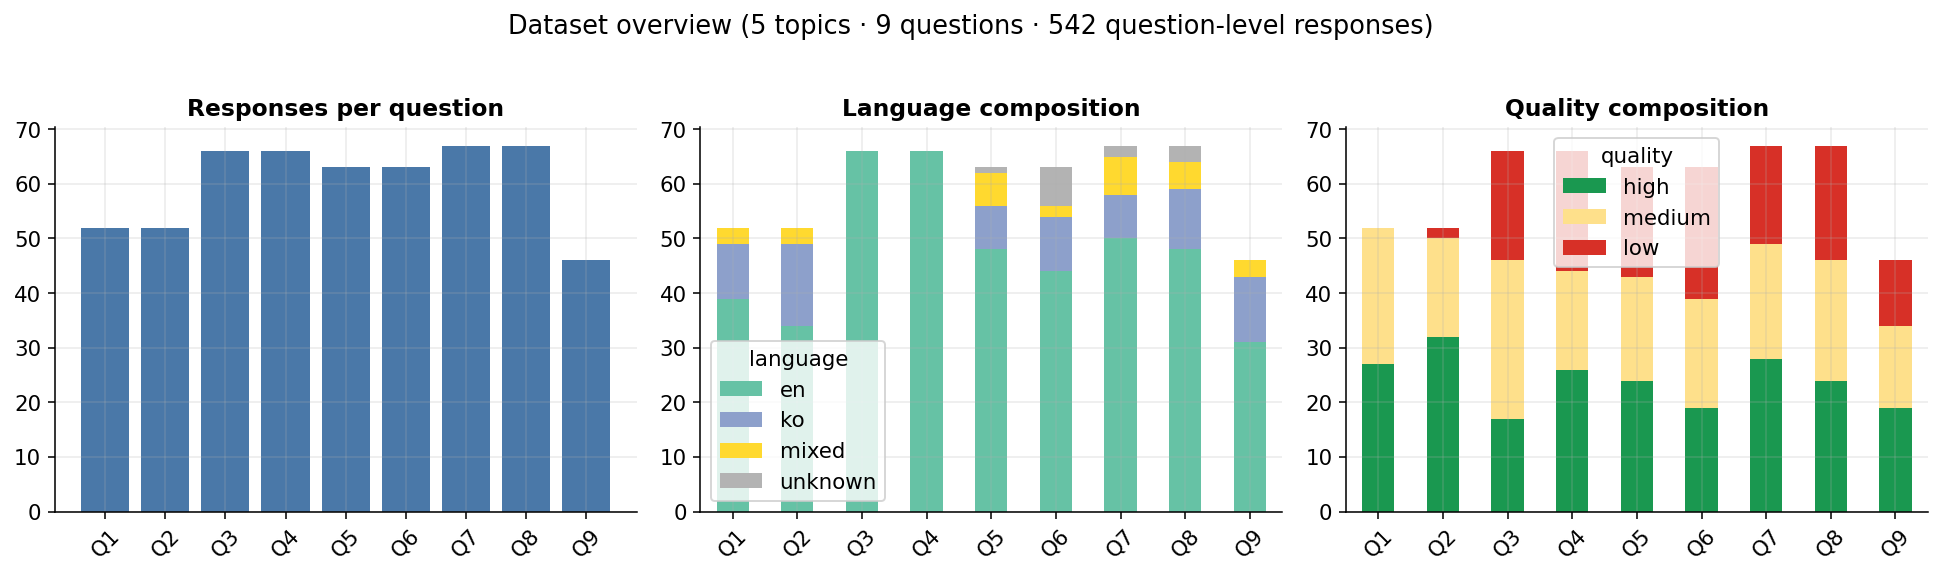
\includegraphics[width=0.92\textwidth]{fig6_data_overview.png}
  \caption{Dataset overview: responses per question, language mix, and quality flags.}
  \label{fig:data}
\end{figure*}

\subsection{Content-fixed, style-coached generation}
The generator (GPT-5-mini, served via the course ELICE API) differs from the
preprocessing model (Claude), so the generator is never its own judge. For every human
answer we generate one LLM answer (1:1, paired by id) that must cover \emph{that human's
keywords}---content is thus held fixed in \emph{every} round. Only a style instruction
changes:
\begin{itemize}\setlength\itemsep{0pt}
  \item \textbf{R0} (naive): keywords only, no style coaching---GPT's default voice.
  \item \textbf{R1} (light): ``write like an undergraduate jotting a quick note.''
  \item \textbf{R2} (aggressive): short, first-person, fragments allowed, no definitions,
        one personal example.
\end{itemize}
Persona, temperature and top-$p$ are fixed across rounds; only the style text varies, so
\emph{every} $\Delta$AUC is a pure style effect. Coaching directions are
\emph{data-driven}: e.g.\ our measurements show naive GPT \emph{under}-hedges relative to
humans, so R2 is told to hedge \emph{more} (the opposite of our initial intuition).

\subsection{Two disjoint style representations}
\textbf{STYLE7} --- seven interpretable surface features: word count, mean word/sentence
length, lexical diversity, first-person ratio, hedging ratio, comma density. These are the
``tells'' the prompt targets. \textbf{STYLO} --- a stylometric vector~\cite{mosteller1964,stamatatos2009}: relative
function-word frequencies, character 3-grams (top 200), and punctuation density. The prompt
never names these. We \emph{assert} the two feature sets share no token (first-person words,
hedge unigrams and the comma are removed from STYLO) so STYLO is a genuinely independent
judge.

\subsection{Technique \textcircled{1}: Classification}
We train human(0) vs.\ LLM(1) classifiers (logistic regression + gradient boosting)
\emph{per question} (never pooled), with 5-fold AUC, a length-only baseline, bootstrap
$95\%$ CIs and label-shuffle permutation tests. For the round comparison we use a
\textbf{leakage-proof} protocol: lock $30\%$ of humans, \emph{freeze} the classifier
trained on the other $70\%$ + R0, and score the held-out humans vs.\ R0/R1/R2 on that frozen
target (20 random splits, per question).

\subsection{Technique \textcircled{2}: Outlier detection}
Independently of the classifier, we fit a Local Outlier Factor (LOF)~\cite{breunig2000} on the LLM answers'
STYLO vectors and score each human by distance from that ``LLM manifold.'' Humans that
remain far from even the best-imitating round are candidate \emph{uncopyable} human
signatures. LOF is distance-based, so it is not a re-run of Technique~\textcircled{1}.

% =====================================================================
\section{Results}
% =====================================================================

\subsection{Style encodes topic $\Rightarrow$ evaluate per question}
Using humans only, style features predict \emph{which question} a response answers with
macro-AUC $0.82$ (STYLE7) and $0.96$ (STYLO) vs.\ chance $0.5$ (Fig.~\ref{fig:confound}).
Style therefore carries topic, not just authorship; pooling questions would let a classifier
cheat on topic. We evaluate strictly per question.

\subsection{Validity: negative control}
Splitting humans into two random groups yields human-vs-human AUC $\approx 0.5$
(Fig.~\ref{fig:negctrl}); shuffling labels collapses every score to chance. Our pipeline does
not manufacture signal from noise.

\begin{figure}[t]
  \centering
  \begin{subfigure}{0.49\columnwidth}
    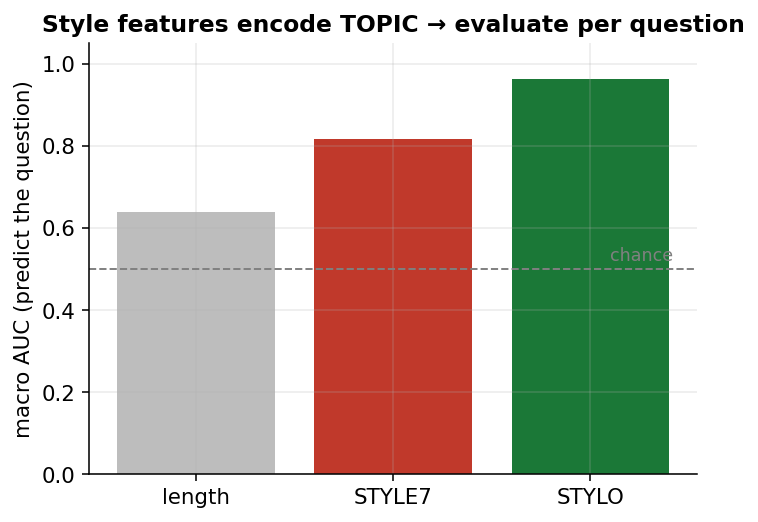
\includegraphics[width=\textwidth]{fig5_topic_confound.png}
    \caption{Topic confound}\label{fig:confound}
  \end{subfigure}\hfill
  \begin{subfigure}{0.49\columnwidth}
    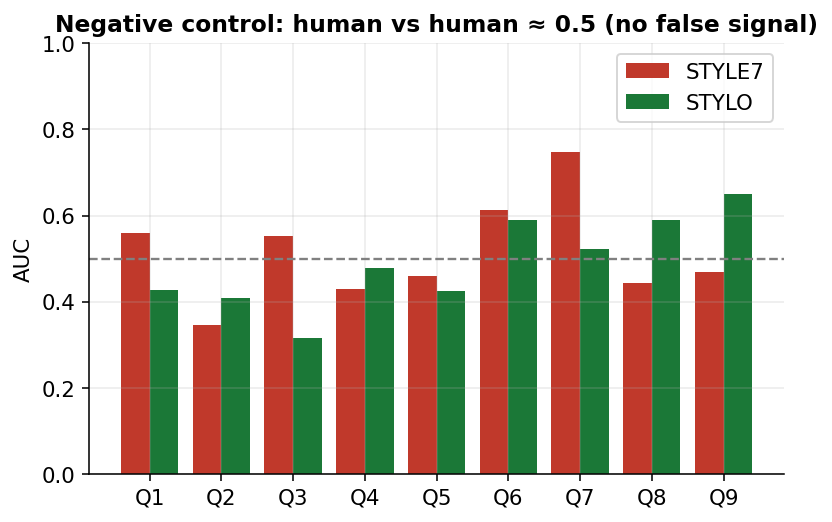
\includegraphics[width=\textwidth]{fig7_negative_control.png}
    \caption{Negative control}\label{fig:negctrl}
  \end{subfigure}
  \caption{Methodology checks: (a) style predicts the question, so we never pool;
  (b) human-vs-human is $\approx 0.5$, so the measure is valid.}
\end{figure}

\subsection{What is the ``LLM tell,'' and how coaching moves it}
Naive R0 is verbose, polished and impersonal: $\sim$6$\times$ longer than humans
(244 vs.\ 41 words), longer sentences, essentially \emph{zero} hedging (0.000 vs.\ 0.004) and
a quarter of the first-person rate (Table~\ref{tab:feats}). Coaching moves every feature
toward---and then \emph{past}---the human value: R2 is shorter, more first-person, hedges
$5\times$ more than humans, and almost never uses commas (Fig.~\ref{fig:feats}). Surface
style is fully controllable, to the point of caricature.

\begin{figure*}[t]
  \centering
  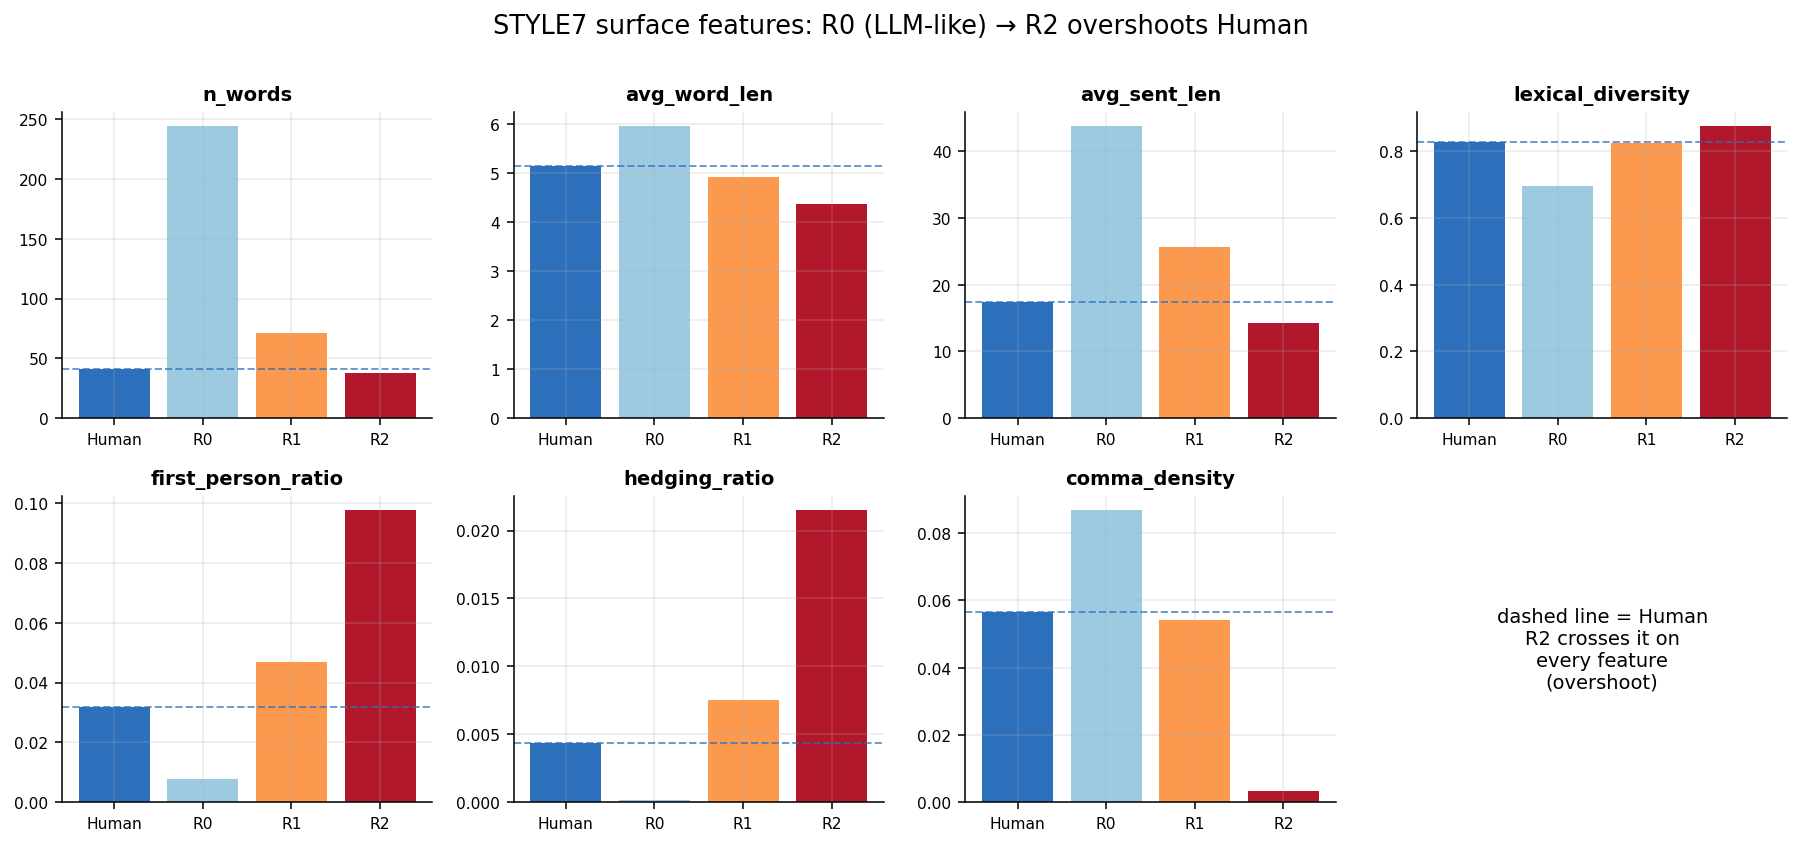
\includegraphics[width=0.92\textwidth]{fig2_style7_feature_trajectory.png}
  \caption{Each STYLE7 feature across Human / R0 / R1 / R2. The dashed line is the human
  mean; R2 \emph{overshoots} it on every feature.}
  \label{fig:feats}
\end{figure*}

\begin{table}[t]\centering\small
  \caption{STYLE7 feature means (English-original set).}
  \label{tab:feats}
  \begin{tabular}{lrrrr}
    \toprule
    feature & Human & R0 & R1 & R2 \\
    \midrule
    n\_words            & 41.3 & 244.3 & 71.1 & 38.0 \\
    avg\_sent\_len      & 17.4 & 43.8  & 25.6 & 14.2 \\
    first\_person\_ratio& 0.032& 0.008 & 0.047& 0.097 \\
    hedging\_ratio      & 0.004& 0.000 & 0.008& 0.021 \\
    comma\_density      & 0.057& 0.087 & 0.054& 0.003 \\
    \bottomrule
  \end{tabular}
\end{table}

\subsection{Headline: surface breaks, signature holds}
Against the frozen R0 classifier on held-out humans (Table~\ref{tab:traj},
Fig.~\ref{fig:auc}), STYLE7 collapses $0.999 \rightarrow 0.079$: below $0.5$ means the
detector now rates R2 as \emph{more human than humans} (the overshoot, inverted). Yet the
\emph{independent} STYLO judge still separates the same R2 answers at AUC $0.776$. Two judges,
identical answers, opposite verdicts: \textbf{surface style closes, the stylometric signature
does not.}

\begin{table}[t]\centering\small
  \caption{Held-out AUC trajectory (frozen R0 classifier) and the LOF outlier rate.}
  \label{tab:traj}
  \begin{tabular}{lccc}
    \toprule
    & R0 & R1 & R2 \\
    \midrule
    STYLE7 AUC (targeted)      & 0.999 & 0.629 & \textbf{0.079} \\
    STYLO AUC (independent)    & 0.991 & 0.926 & \textbf{0.776} \\
    LOF: \% humans outside LLM & 100\% & 83\%  & \textbf{59\%}  \\
    \bottomrule
  \end{tabular}
\end{table}

\begin{figure}[t]
  \centering
  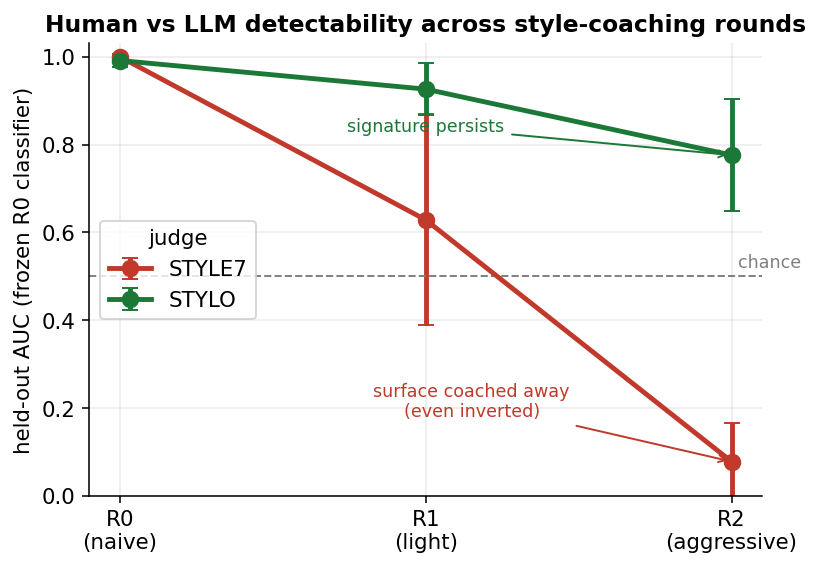
\includegraphics[width=0.86\columnwidth]{fig1_auc_trajectory.png}
  \caption{The headline result. STYLE7 (targeted) is coached away and inverts; STYLO
  (independent) stays well above chance.}
  \label{fig:auc}
\end{figure}

\subsection{Two techniques converge}
Outlier detection corroborates classification from a distance-based angle: as imitation
improves, the share of humans outside the LLM STYLO cloud falls $100\%\rightarrow83\%\rightarrow59\%$,
but a clear majority remains outside even at R2 (Fig.~\ref{fig:converge}). A 2-D projection of
the STYLO space shows the mimic round R2 forming its own cluster, never merging into the
dispersed human region (Fig.~\ref{fig:pca}).

\begin{figure}[t]
  \centering
  \begin{subfigure}{0.49\columnwidth}
    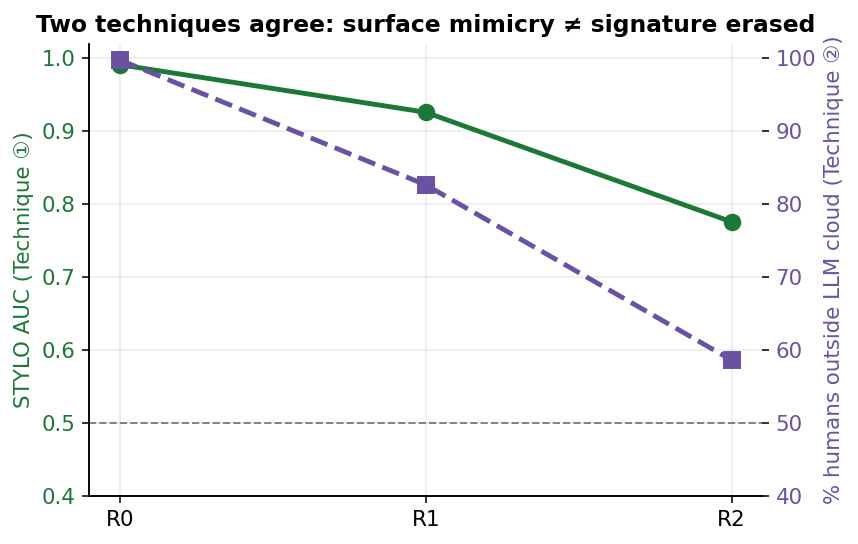
\includegraphics[width=\textwidth]{fig3_two_technique_convergence.png}
    \caption{Both techniques}\label{fig:converge}
  \end{subfigure}\hfill
  \begin{subfigure}{0.49\columnwidth}
    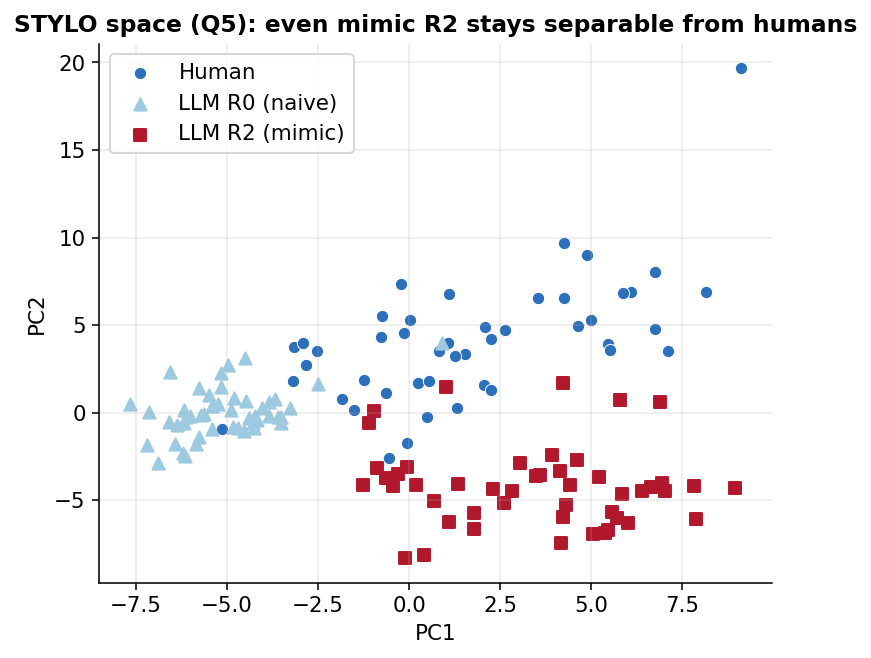
\includegraphics[width=\textwidth]{fig4_stylo_pca_Q5.png}
    \caption{STYLO space (Q5)}\label{fig:pca}
  \end{subfigure}
  \caption{Classification and outlier detection agree that the signature survives imitation.}
\end{figure}

\subsection{Robustness}\label{sec:robust}
Varying the analysis set across four definitions---translation-included vs.\
English-original, and strict vs.\ inclusive quality filtering---leaves the conclusion intact:
STYLE7@R2 $\approx 0.07$ and STYLO@R2 $\in[0.76,0.78]$ throughout (Fig.~\ref{fig:robust}).
Critically, English-original ($0.78$) $\approx$ translation-included ($0.76$), so the
surviving signature is \emph{not} an artifact of machine translation. And because R2 and
humans are length-matched ($38$ vs.\ $41$ words), the residual STYLO signal is not a length
artifact either.

\begin{figure}[t]
  \centering
  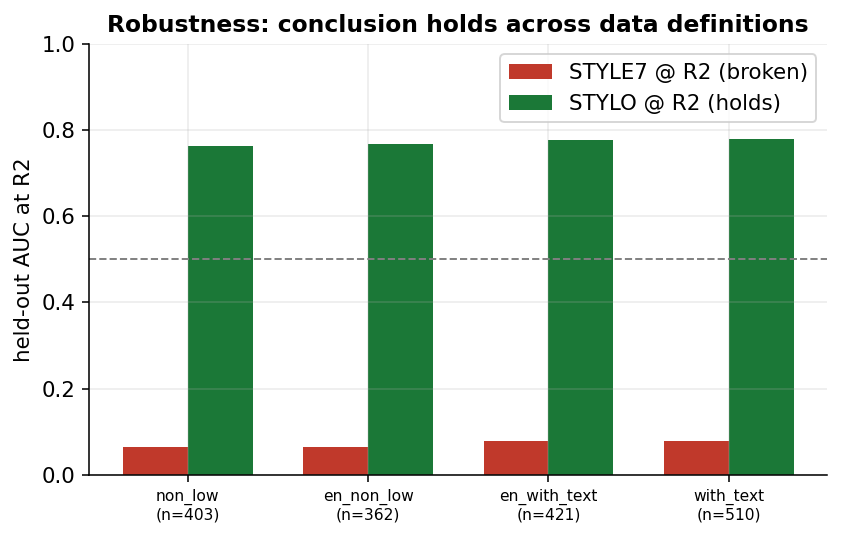
\includegraphics[width=0.86\columnwidth]{fig8_robustness.png}
  \caption{The ``surface breaks, signature holds'' pattern is stable across data definitions.}
  \label{fig:robust}
\end{figure}

% =====================================================================
\section{Discussion and Conclusion}
% =====================================================================
\textbf{Findings.} (1) Surface style (length, person, hedging, punctuation) is fully
prompt-controllable---an LLM told to imitate a student will overshoot real students. (2) A
stylometric signature (function-word and punctuation rhythm) is \emph{not} prompt-controllable
and remains detectable (AUC $0.78$; $59\%$ of humans irreducibly outside) even under
aggressive coaching. (3) Two independent techniques and four data definitions agree.

\textbf{Insight.} ``Looks human'' (surface) and ``is statistically human'' (signature) come
apart. Surface mimicry is therefore weak evidence of genuine human-likeness; the irreducible
signal is the unconscious, sub-lexical fingerprint.

\textbf{Limitations.} STYLO is not perfectly immune (it drops $0.99\rightarrow0.78$); its
residual is real but partial. R2 is a \emph{caricature} (overshoot), so we claim ``surface
\emph{tells} neutralized,'' not ``student faithfully reproduced.'' Our humans are Korean
undergraduate ESL writers and the LLM is native-like, so part of the residual may be an
ESL$\leftrightarrow$native register difference; within our research question (can the LLM imitate
\emph{these} students) this is a property of the population, not a confound, and we do not
generalize beyond it.

\textbf{Future work.} Add an ESL-conditioned generation round and a native-speaker corpus to
separate ``human'' from ``non-native'' signal; exploit the 1:1 pairing for a paired test;
test additional generators.

\textbf{Conclusion.} When content is fixed and only style is coached, prompt-level control
erases the surface tells of LLM text but cannot erase its stylometric signature---that
signature is the component of human writing an LLM cannot yet fake.

% =====================================================================
\section{Roles and Responsibilities}
% =====================================================================
\begin{table}[H]\centering\small
  \begin{tabular}{ll}
    \toprule
    Member & Responsibility \\
    \midrule
    A & Preprocessing pipeline, master dataset \\
    B & Generation (R0--R2), prompt design \\
    C & Classification, round evaluation \\
    D & Outlier detection, figures, report \\
    \bottomrule
  \end{tabular}
  \caption{Tentative; finalize before submission.}
\end{table}

\textbf{Reproducibility.} All parameters live in \texttt{config/config.yaml}; the pipeline runs
end-to-end from the master JSON with \texttt{generate.py} $\rightarrow$ \texttt{classify.py}
$\rightarrow$ \texttt{round\_eval.py} $\rightarrow$ \texttt{outlier\_lof.py} $\rightarrow$
\texttt{05\_figures.py}. All models use scikit-learn~\cite{pedregosa2011}.

\bibliographystyle{plain}
\bibliography{references}

\end{document}
